\documentclass{stdlocal}
\begin{document}
\section{Evaluation and Results} % (fold)
\label{sec:evaluation}
  \autocite{compiler-explorer,intel-intrinsics-guide,perfevent,vandevoorde2018,meyers2014}

  \subsection{Statistical Performance} % (fold)
  \label{sub:statistical_performance}
    From a theoretical point of view, interleaving multiple streams of random numbers based on multiple instances of the same generator should not reduce the randomness of the output, such that test suites will be able to measure it.
    Using multiple instances the state of the vectorized PRNG becomes four times as big as the scalar variant.
    According to \textcite{oneill-blog-toobig}, creating a larger state will even make a weak generator stronger concerning its statistical performance.
    We will run the tests to confirm this.
  % subsection statistical_performance (end)

  \begin{figure}
    \center
    \begin{subfigure}[b]{\textwidth}
      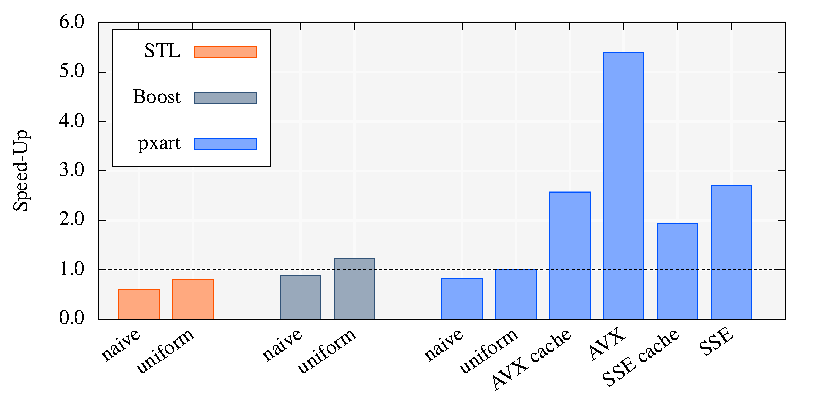
\includegraphics[width=\textwidth]{plots/monte_carlo_pi_laptop_mt19937.pdf}
      \caption{MT19937}
    \end{subfigure}

    \begin{subfigure}[b]{\textwidth}
      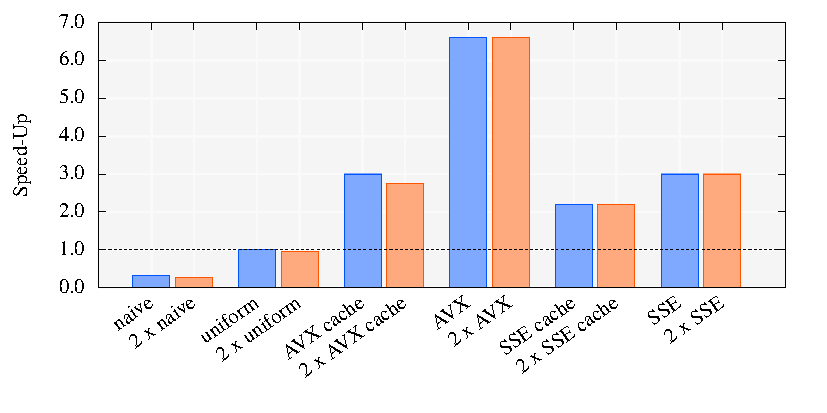
\includegraphics[width=\textwidth]{plots/monte_carlo_pi_laptop_xrsr128p.pdf}
      \caption{Xoroshiro128+}
    \end{subfigure}

    \begin{subfigure}[b]{\textwidth}
      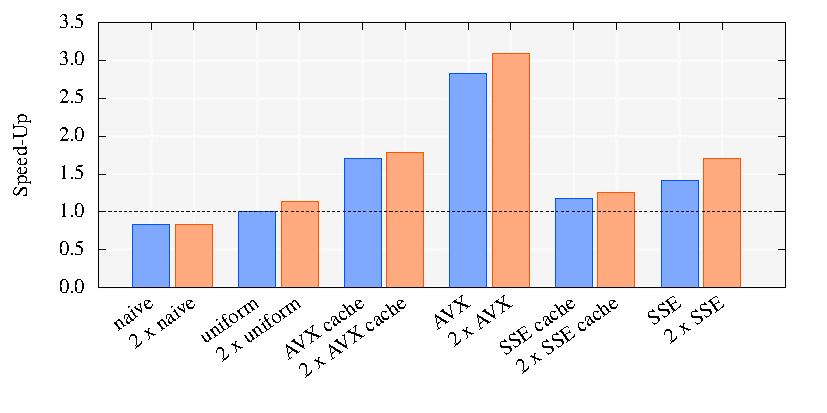
\includegraphics[width=\textwidth]{plots/monte_carlo_pi_laptop_msws.pdf}
      \caption{MSWS}
    \end{subfigure}
    \caption{}
  \end{figure}

  \begin{table}
    \center
    \caption{}
    \footnotesize
    \renewcommand{\arraystretch}{1.2}
    \subimport{tables/}{monte_carlo_pi_laptop.tex}
  \end{table}
% section evaluation (end)
\end{document}